% nastavenia prostredia
\documentclass[12pt,a4paper,titlepage,final]{report}
\usepackage[utf8]{inputenc}
\usepackage[T1, IL2]{fontenc}
\usepackage{graphicx}
\usepackage{epstopdf}
\usepackage[margin=2cm]{caption}
\usepackage[top=3cm, left=1cm, right=1cm, text={17cm, 24cm}, ignorefoot]{geometry}
\usepackage{color}
\usepackage{url}
\usepackage[bookmarksopen,colorlinks,plainpages=false,urlcolor=blue,unicode]{hyperref}
\usepackage{setspace}
\usepackage[czech]{babel}
\singlespacing

\begin{document}
	% define
	\def\authora{Michal Riša}
	\def\authorb{Pavel Macenauer}
	\def\emaila{xbures19@stud.fit.vutbr.cz}
	\def\emailb{xmacen02@stud.fit.vutbr.cz}
	\def\docname{Počítačová grafika}
	\def\projname{Raytracing na CUDA}
	% titulna strana
	\begin{titlepage}

\vspace*{1cm}

\begin{figure}
  \centering
  
\includegraphics[height=6cm]{images/fit.pdf}
\end{figure}

\vspace*{5mm}

\begin{center}
\begin{Large}
Projekt do předmětu PGR -- Počítačová grafika
\end{Large}
\end{center}

\vspace*{5mm}

\begin{center}
\begin{Huge}
CUDA Raytracer \\
\end{Huge}
\end{center}

\vspace*{1cm}

\begin{center}
\begin{Large}
\today
\end{Large}
\end{center}

\vfill

\begin{flushleft}
\begin{large}
\begin{tabular}{ll}

\bf Řešitelé:\hspace{3mm}
& Jan Bureš (\verb_xlogin00@stud.fit.vutbr.cz_) \\
& Pavel Macenauer (\verb_xmacen02@stud.fit.vutbr.cz_) \\
& Fakulta Informačních Technologií \\
& Vysoké Učení Technické v~Brně

\end{tabular}
\end{large}
\end{flushleft}

\end{titlepage}

% vim:set ft=tex expandtab enc=utf8:

	% kapitoly
	\newpage
	\pagestyle{plain}
	\pagenumbering{arabic}
	\setcounter{page}{1}
	\setcounter{secnumdepth}{-1}
	\setlength{\parindent}{1cm}	

%---------------------------------------------------------------------------
\section{Zadání}

Zde napište informace k zadání (nejde jen o přepis toho, co je na webu;
komentujte vaše vlastní zpřesnění zadání, zaměření, důrazy, pojetí atd.). Text
strukturujte, použijte odrážky, číslování$\ldots$

Rozsah: cca 10 odrážek

%---------------------------------------------------------------------------
\section{Použité technologie}

Zde vypište, jaké technologie vaše řešení používá – co potřebuje k běhu, co
jste použili při tvorbě, atd. Text strukturujte, použijte odrážky,
číslování$\ldots$

Rozsah: cca 7 odrážek
Minimální požadavky pro spuštění programu:
Použité technologie:
\begin{itemize}
	\item CUDA 3.0
	\item OpenGL 4
	\item GLM
	\item Glut
	\item Glew
\end{itemize}
\subsection{Při tvorbě jsme použili tyto programy:}
\begin{itemize}
	\item Visual Studio 2012 + NSight
	\item GitHub
\end{itemize}
%---------------------------------------------------------------------------
\section{Použité zdroje}

Zde vypište, které zdroje jste použili k tvorbě: hotový kód, hotová data
(obrázky, modely, $\ldots$), studijní materiály. Pokud vyplyne, že v projektu
je použit kód nebo data, která nejsou uvedena tady, jedná se o závažný problém
a projekt bude pravděpodobně hodnocen 0 body.

Rozsah: potřebný počet odrážek
Studijní zdroje:
\begin{itemize}
\item Přednáška PGR (Realistické zobrazování I - Ray Tracing)
\item \href{https://www.fit.vutbr.cz/study/courses/PGR/private/Aurelius.zip}{Ray-tracer Aurelius}
\item Přednáška PGP (Fotorealistcké zobrazování, optimalizace sledování paprsku)
\item \href{http://docs.nvidia.com/cuda}{CUDA Toolkit Documentation}
\end{itemize}
Doplňujicí zdroje:
\begin{itemize}
\item \href{http://cs.wikipedia.org/wiki/Phong%C5%AFv_osv%C4%9Btlovac%C3%AD_model}{Phongův osvětlovací model}
\item \href{http://stackoverflow.com/questions/19013156/how-does-cuda-4-0-support-recursion}{Rady ohledně rekurze v CUDA}
\item \href{http://www.3dmuve.com/3dmblog/?p=182}{Bounding Volume Hierarchies (BVH) – A brief tutorial on what they are and how to implement them}
\item \href{http://cuda-programming.blogspot.cz/2013/01/what-is-constant-memory-in-cuda.html}{What is constant memory in CUDA?}
\item \href{http://cg.alexandra.dk/2009/08/10/triers-cuda-ray-tracing-tutorial/}{Triers CUDA ray tracing tutorial}
\end{itemize}
%---------------------------------------------------------------------------
\section{Nejdůležitější dosažené výsledky}

\begin{center}
	\captionsetup{type=figure}
		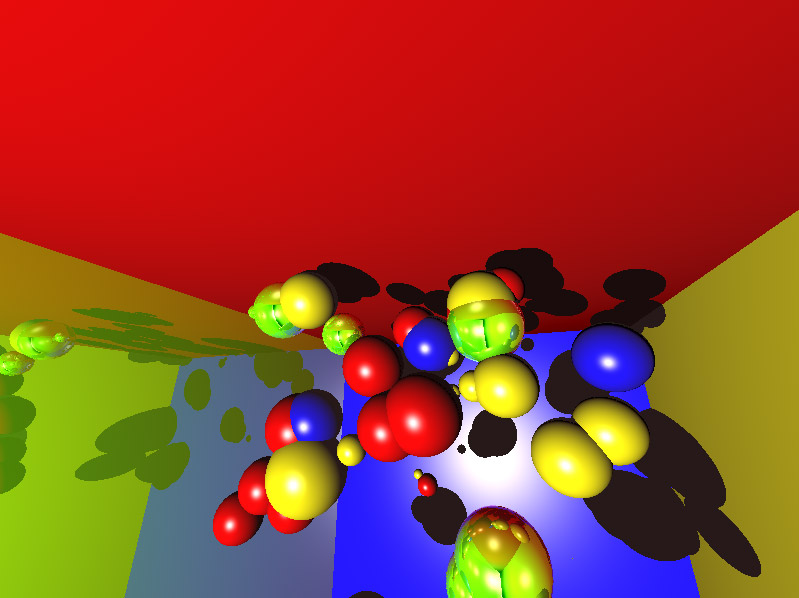
\includegraphics[width=14cm]{images/no-sampling-no-bvh.jpg}
	\captionof{figure}{Vygenerovaná scéna bez využití jakéhokoliv urychlení}
	
		\captionsetup{type=figure}
		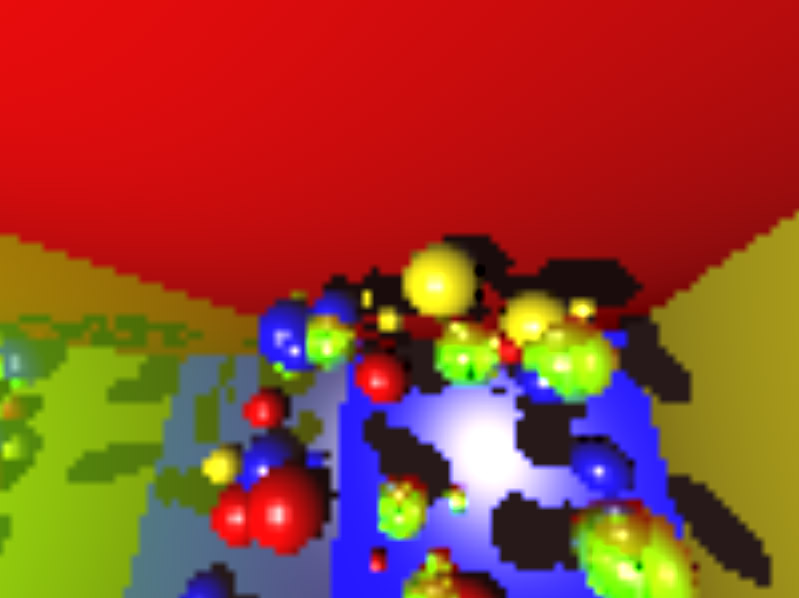
\includegraphics[width=14cm]{images/with-sampling-no-bvh.jpg}
	\captionof{figure}{Vygenerovaná scéna s využitím bilineární samplování}
\end{center}

%---------------------------------------------------------------------------
\section{Ovládání vytvořeného programu}

Stručně popište, jak se program ovládá (nejlépe odrážky rozdělené do
kategorií). Pokud se ovládání odchyluje od zkratek a způsobů obvykle
používaných v okýnkových nadstavbách operačních systémů, zdůvodněte, proč se
tak děje.

Rozsah: potřebný počet odrážek

%---------------------------------------------------------------------------
\section{Zvláštní použité znalosti}

Uveďte informace, které byly potřeba nad rámec výuky probírané na FIT.
Vysvětlete je pomocí obrázků, schémat, vzorců apod. 

Rozsah: podle potřeby 

%---------------------------------------------------------------------------
\section{Rozdělení práce v týmu}

\begin{itemize}
\item xbures19: Phongův osvětlovací model, úprava bilinear sampling, část raytraceru 
\item xmacen02: Základní kostra programu, optimalizace využitých paměťových jednotek, bilinear sampling, část raytraceru 
\end{itemize}
Pokud to bude vhodné, použijte odrážky místo souvislých vět.

Rozsah: co nejstručnější tak, aby bylo zřejmé, jak byla dělena práce a za co v
projektu je kdo zodpovědný.

%---------------------------------------------------------------------------
\section{Co bylo nejpracnější}

Popište, co vám při řešení nejvíce komplikovalo život, s čím jste se museli
potýkat, co zabralo čas.

Rozsah: 5-10 řádků

Na celé práci bylo asi nejložitější upravit algoritmus sledování paprsku tak,
aby fungoval na architektuře CUDA. Dále pak správné rozdělení vláken do warpů 
a rozhodnout, který druh paměti použít pro které proměnné. Mno času bylo zapotřebí  
také věnovat rekurzi, kterou by sice CUDA měla podporovat od verze 3.0,  
ovšem stále program havaroval kvůli přetečení zásobníku.

%---------------------------------------------------------------------------
\section{Zkušenosti získané řešením projektu}

Popište, co jste se řešením projektu naučili. Zahrňte dovednosti obecně
programátorské, věci z oblasti počítačové grafiky, ale i spolupráci v týmu,
hospodaření s časem, atd.

Rozsah: formulujte stručně, uchopte cca 3-5 věcí

Naučili jsme se více o architektuře CUDA, vyzkoušeli si implementovat phongův osvětlovací model a
raytracer. Dále jsme si prostudovali možné algoritmické optimalizace raytraceru.

%---------------------------------------------------------------------------
\section{Autoevaluace}

Ohodnoťte vaše řešení v jednotlivých kategoriích (0 – nic neuděláno,
zoufalství, 100\% – dokonalost sama). Projekt, který ve finále obdrží plný
počet bodů, může mít složky hodnocené i hodně nízko. Uvedení hodnot blízkých
100\% ve všech nebo mnoha kategoriích může ukazovat na nepochopení problematiky
nebo na snahu kamuflovat slabé stránky projektu. Bodově hodnocena bude i
schopnost vnímat silné a slabé stránky svého řešení.

\paragraph{Technický návrh (60\%):} (analýza, dekompozice problému, volba
vhodných prostředků, $\ldots$) 
Stručně (1-2 řádky) komentujte hodnocení. 

\paragraph{Programování (70\%):} (kvalita a čitelnost kódu, spolehlivost běhu,
obecnost řešení, znovupoužitelnost, $\ldots$)
Stručně (1-2 řádky) komentujte hodnocení. 

\paragraph{Vzhled vytvořeného řešení (80\%):} (uvěřitelnost zobrazení,
estetická kvalita, vhled GUI, $\ldots$)
Stručně (1-2 řádky) komentujte hodnocení. 
Scéna vypadá docela pěkně.

\paragraph{Využití zdrojů (80\%):} (využití existujícího kódu a dat, využití
literatury, $\ldots$)
Hodně jsme využil již implementovaný raytracer. Trochu méně jsme pak použiváli dostupnou literaturu.

\paragraph{Hospodaření s časem (60\%):} (rovnoměrné dotažení částí projektu,
míra spěchu, chybějící části řešení, $\ldots$)
Bylo by vhodné začít dřív s implementací.

\paragraph{Spolupráce v týmu (95\%):} (komunikace, dodržování dohod, vzájemné
spolehnutí, rovnoměrnost, $\ldots$)
Stručně (1-2 řádky) komentujte hodnocení. 
od začátku jsme komunikovali ohledně podmínek spolupráce. Následné programování pak probíhalo bez problémů.

\paragraph{Celkový dojem (85\%):} (pracnost, získané dovednosti, užitečnost,
volba zadání, cokoliv, $\ldots$)
Stručně (5-10 řádků) komentujte hodnocení. 

%---------------------------------------------------------------------------
\section{Doporučení pro budoucí zadávání projektů}

Co vám vyhovovalo a co nevyhovovalo na organizaci projektů? Které prvky by měly
být zachovány, zesíleny, potlačeny, eliminovány?
Určitě bychom uvítali zpřesnění zadání (stačili by stručné body).

%---------------------------------------------------------------------------
\section{Různé}

Ještě něco by v dokumentaci mělo být? Napište to sem! Podle potřeby i založte
novou kapitolu.

\end{document}
% vim:set ft=tex expandtab enc=utf8:
